%===================================== CHAP 3 =================================

\chapter{Implementation}

\textit{Detailed description of the web interface and its structure as well as case study, this was missing from the specialization project. \\
\noindent Present the technology used (might have to reword the name of this chapter). \\
\noindent Include several typical software development diagrams.}

\section{Visualization Tool}

\subsection{Prototype}

This section will describe the prototype of the web interface to be improved as well as some pointers on what should be implemented in the next version.

\subsubsection{Description}

\noindent The prototype provides all the basic user functionality for creating a user, and logging in and out, including validation of user name and password. A user can upload Python scripts from their computer to the server, and tag them with various topics to make them easier to search for, using the search bar on the page showing all uploaded scripts. \\

\noindent By selecting a specific script, the user can view the code, add tags to, delete, and of course run, the script. A separate menu tab for visualizations provides the user with visualizations of the data produced while running. The only visualization techniques implemented are the training progress and layer activations laid out after each other on a single page. The training progress includes two separate plots showing accuracy and loss over batch, while the layer activations are shown for each single layer of the network defined in the script.

\subsubsection{Planned Improvements}

The overall purpose will be to add more functionality with the goal of improving the user's understanding of the network. This may be new visualization techniques, training process statistics, better presentations of data, and more user controls. Another useful addition can be allowing the user more flexibility and make the visualizations more interactive.

\subsection{System Development Methodology}

The development of the visualization tool has been carried out by a team consisting of the two of us, with no specific set of roles. Because of the small team size, we did not see the need for a dedicated project manager. Both of us were involved in designing the architecture and interface, as well as implementing and testing the system, giving us great knowledge of the whole system. Still, we maintained an efficient workflow by dividing the programming task into two main responsibility areas, one for each of us:
\begin{enumerate}
    \item Visualizing data using the selected visualization library and incorporating these into the user interface
    \item Implementing visualization techniques and creating networks to illustrate the use of the tool with the chosen deep learning library
\end{enumerate}

\noindent The development process itself did not follow any strict guidelines, but included several elements from Agile methods. It has been an iterative and incremental process, starting with the existing prototype of the system that only implemented two of the visualization techniques in a very simple manner. Based on our own testing as well as feedback from the customer, which in this case is our supervisors, functionality were added and adjustments were made in order to obtain a new and improved prototype. This process was repeated until we reached a satisfactory system according to the initial requirements. An example of the iterative part of the process is when we decided to replace the old visualization library with a new one that better suited our needs. An example of the incremental part of the process is when our supervisors expressed the wish for a way for the user to be able to upload an image to be used in producing some of the visualizations. Other concepts from Agile development that were put into use are code review, pair programming, and the use of a backlog to get an overview of the requirements.

\subsection{Focus Quality Attributes}

\subsubsection{Modifiability}

An important aspect of the system design of the visualization tool is to make sure that any part can be easily replaced. For instance, it should not be too difficult to alter the system to use a different deep learning library than the one employed in our implementation. This requires thorough consideration when designing the architecture, and typically calls for a module-based architecture with each module being loosely coupled, meaning that it should interact with as few of the other modules as possible.

\subsubsection{Usability}

Not only should the interface be simple and easy to navigate for the user, but the actual installation of the program and the adaption of the user's deep learning scripts to the tool, should be without much trouble. A thorough user manual and documentation of the API is the key to obtaining this kind of usability. Preferably, we would want any ANN to run in our program without problems, but it is near to impossible to generalize this much. The main goal was thus to support the most commonly used networks, but at the same time, as the previous section mentions, easily allow for extending the system to work with different kinds of ANNs.

\subsection{Technology Decisions}

\subsubsection{Flask}

Flask is a web framework written in Python, used to build simple web applications. It is a micro-framework, meaning that it has very few dependencies to external libraries. It provides you with only the basic tools needed to create a web application, and is therefore very lightweight. There exists many plugins that can be added for an increased range of functionality. Since the focus of our visualization tool is not the web page itself, but rather its capabilities in terms of visualization techniques, Flask is the perfect choice. It allowed us to quickly set up an application and implement a basic user system and upload functionality.

\subsubsection{SQLite}

Very lightweight and easy to include in simple desktop apps that could make use of a database. Do not really need to store much data. Simple relational data. Not an important part of the application. Lightweight. Not a lot of connections.

\subsubsection{Keras}

Keras is a high-level neural networks library that can run on top of either TensorFlow or Theano. Its purpose is to provide a way to quickly and easily create models and start experimenting. It is very minimalistic, providing only enough to achieve an outcome, while still allowing for extensibility by making it easy to add and use new modules within the framework. Keras provides the user with several callbacks, i.e. sets of functions to be applied at giving stages of the ANN training procedure. It also allows for creating your own custom callbacks, which is perfect for our use case, since we then can create callbacks that produces the data needed for each visualization technique.

\subsubsection{TensorFlow}

Not sure if we need this section. But mention in Keras section, and say whether we support both Theano and TensorFlow?

\subsubsection{Bokeh}

Bokeh is a Python interactive visualization library for modern web browsers. It can easily be embedded into a Flask application, as we will show in a later section. The library is easy to use, and has the flexibility of adding interactions and highly advanced customization. Another benefit is that it is easy to stream large data sets and plot them live. \textit{Something about the drawbacks because it is new.}

A lot of possibilities for adding interactions, easy to stream live plotting of data. Drawbacks are that it is fairly new and still under development. Also probably not the best for handling images.

\subsection{Overview of the Architecture}

As seen in \textbf{Fig. \ref{architecture1}}, the system can be said to consist of five separate modules: Flask, the user storage, the database, Bokeh, and Keras. The Flask module is the very core of the application, and defines the routes (URLs), models and forms of the web page, tying the logic together with HTML templates, CSS and JavaScript into a simple functional web interface. The user storage is where all scripts and images uploaded through the Flask application are stored, as well as text files containing the produced data during training. The database contains metadata about the scripts that is used in the Flask application, such as the owner, when it was uploaded, and the path to the script. The Keras module includes the custom callbacks created for visualization that writes data to the files stored in the user storage. A user applied the wanted callbacks to his or her scripts. It is the Flask application that implements the logic of running these scripts. Finally, the Bokeh module uses the data stored in user storage to create live interactive visualizations, and the Flask application takes care of displaying these on the web page. \\

\noindent \textit{Something about modular approach, that it is good for extensibility, etc.}

% First, the overall architecture. Explain the different modules.
% Then we can focus on some parts of the architecture that we want to "show off".

\begin{figure}[h!]
    \centering
        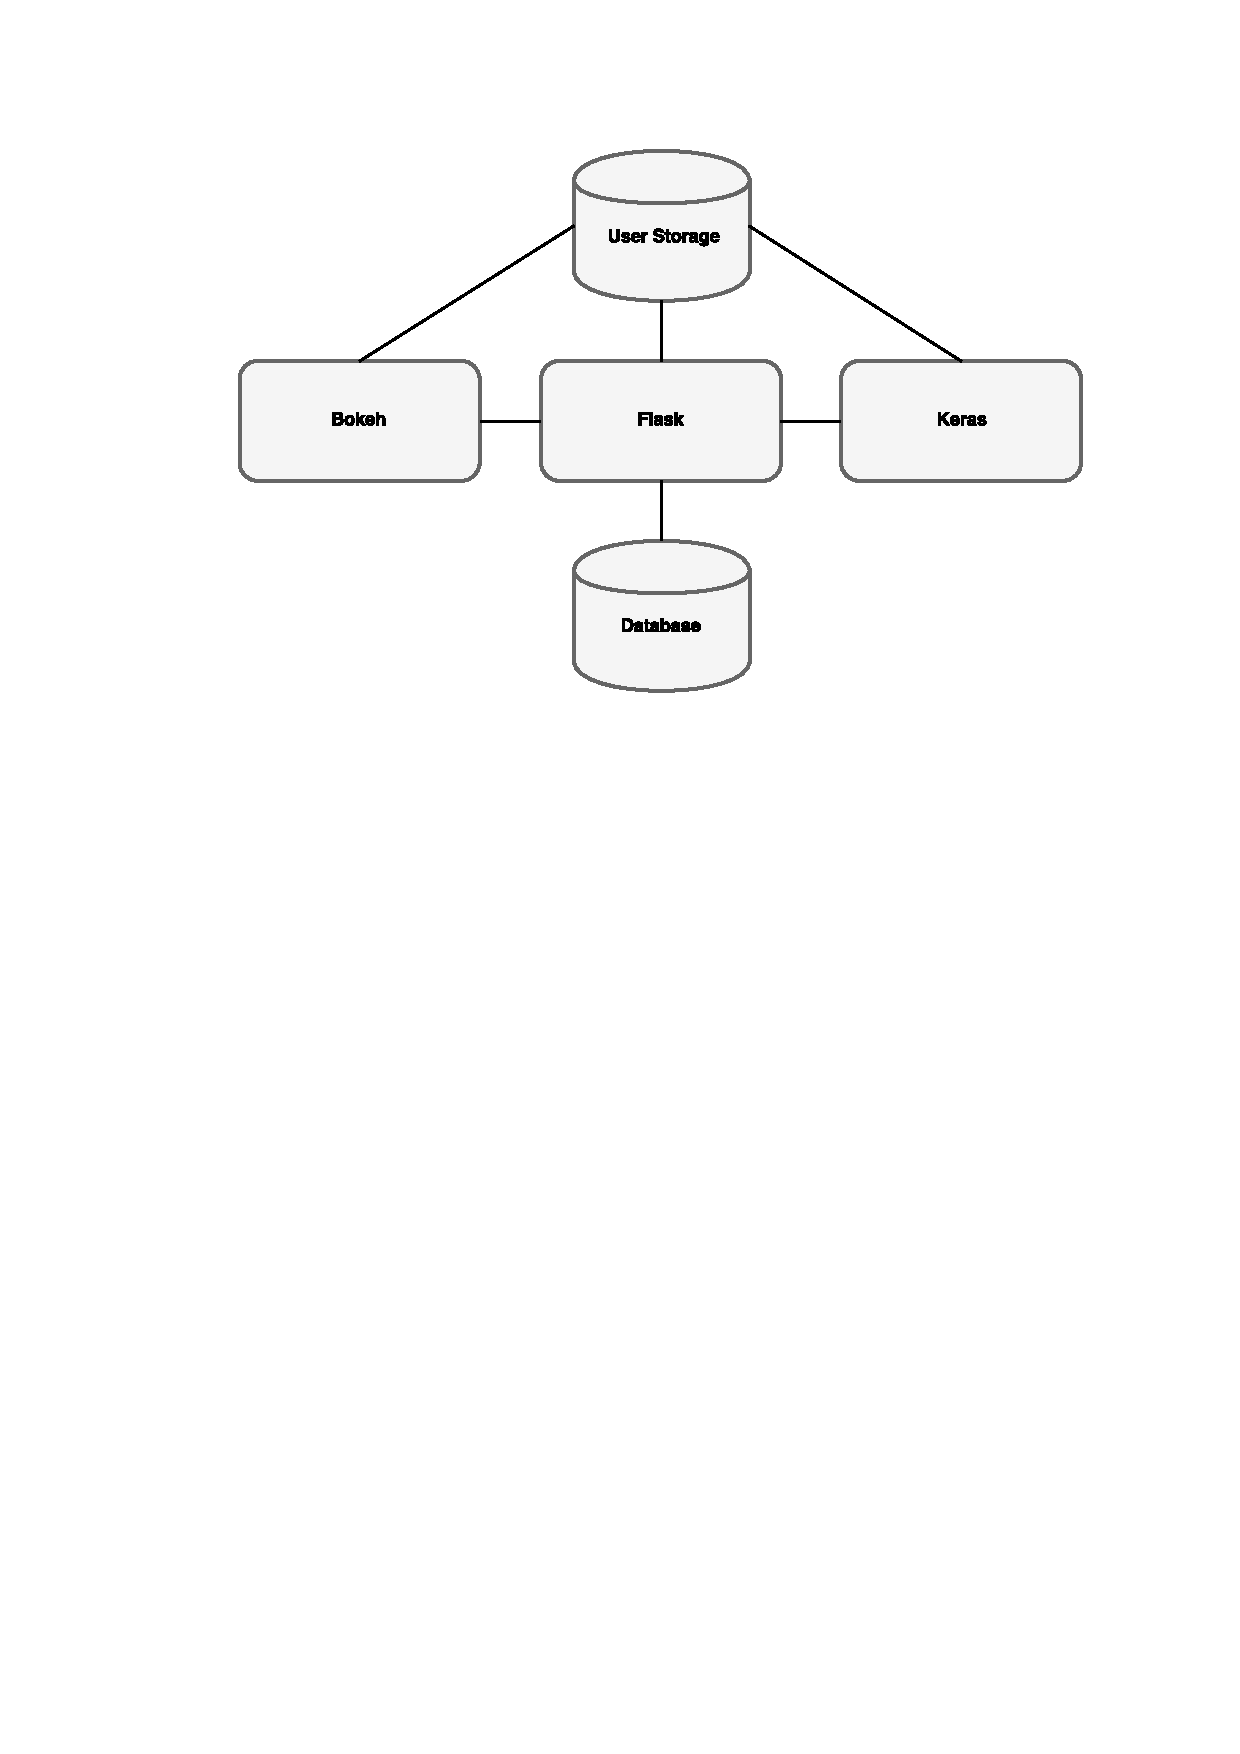
\includegraphics[width=0.7\textwidth]{fig/overall-architecture.pdf}
        \caption{Overall Architecture of the System}
        \label{architecture1}
\end{figure}

% Examples here are the relation between bokeh and flask, flask and keras, flask and the user storage. etc.

\subsection{The Flask Application}

\textbf{Fig. \ref{struct}} shows a high-level overview of the structure of the files included in the Flask application. The static folder serves all the CSS and JavaScript files, while the templates folder contains Jinja2 templates that Flask can render to generate the HTML. The init file contains the instantiation of the Flask application as well as some setup for the database and log in system. The config file configures some parameters for the application, such as the command used to run a python script.\\

\begin{figure}[ht]
\begin{verbatim}
/visualizer
    /static
        /css
        /fonts
        /js
    /templates
        /create_user.html
        /home.html
        /layout.html
        /...
    /__init__.py
    /config.py
    /forms.py
    /helpers.py
    /models.py
    /requirements.txt
    /views.py
    /visualizer.db
\end{verbatim}
\caption{Flask project files}
\label{struct}
\end{figure}

\noindent There are three main files implementing the logic: forms.py, models.py and views.py. They define all the forms, models and views, respectively, of the web page. A form is used to collect user input, for instance while registering a new user, or uploading a script. Models are used to create database objects. Finally, a view defines a URL endpoint, or a route, as well as what HTTP requests it answers to, and determines what should happen when a user arrives at that URL. There is also a helpers file that contains various helper methods.\\

\noindent An actual example of a view from views.py is shown in \textbf{Code \ref{code:2}}. Comments and irrelevant code are removed to simplify the example. Line 1 defines the route of the view, hence the complete URL of this view will be \texttt{localhost:5000/create\_user}. It also defines the HTTP requests to answer to, which is both GET and POST. GET is for just returning the page to register a user, while POST is when a user actually presses the button to register. The code illustrates the use of a form in line 3, in this case a form for creating a new user, which contains the chosen username and password of the new user. Line 5 checks if all fields are valid when a user has submitted (the POST request), while the next line makes sure to alert the user and break the process if the username is alredy taken. If everything this far is fine, line 9 creates a User model consisting of the username and password (the model also takes care of hashing the password) and adds it to the database. Line 13 redirects the user to another view, namely the log in view. If the user has not submitted their form, line 15 makes sure to render the correct template for the user registration page. \\

\begin{listing}[ht]
\begin{minted}
[
frame=lines,
framesep=2mm,
baselinestretch=1.2,
fontsize=\footnotesize,
linenos
]
{python}
@app.route('/create_user', methods=['GET', 'POST'])
def create_user():
	form = CreateUserForm()
	
	if form.validate_on_submit():
		if not unique_username(form.username.data):
			flash('Username is already taken', 'danger')
		else:
			db.session.add(User(form.username.data, form.password.data))
			db.session.commit()
			
			flash('User successfully created', 'success')
			return redirect(url_for('login'))
		
	return render_template('create_user.html', form=form)
\end{minted}
\caption{View for creating a user}
\label{code:2}
\end{listing}

\subsection{Running a Python Script}

The visualization tool allows a user to both start and stop the uploaded python scripts. Functionality for running a script is implemented as a helper function, and is done by executing \texttt{python [file\_path]} in a new subprocess, as seen in \textbf{Code \ref{code:3}}. The actual Python command is determined by a config variable, since it depends on the user's Python installations (e.g. some systems use \texttt{python3} for Python 3.6 and simply \texttt{python} for Python 2.7). The \texttt{stdout} argument specifies the standard output file handle, which is in this case a text file that will be displayed on the web page, so that the user is given easy access to the output of the script. Note that even though \textbf{Fig. \ref{architecture1}} shows a connection between Keras and Flask, the real connection is really between Python and Flask. A user could easily upload a Python script that uses the scikit-learn library or pure TensorFlow, running such a script would not cause any problems. However, if someone wanted to adapt the visualization tool to a whole different programming language, this section of the code would need to be replaced.

\begin{listing}[ht]
\begin{minted}
[
frame=lines,
framesep=2mm,
baselinestretch=1.2,
fontsize=\footnotesize,
linenos
]
{python}
with open(get_output_file(get_current_user(), basename(file_path)), 'w') as f:
	p = subprocess.Popen([PYTHON, file_path], stdout=f)
\end{minted}
\caption{Running a Python script using subprocess}
\label{code:3}
\end{listing}

\subsection{Custom Keras Callbacks}

The custom callbacks are the only part of the visualization tool that are specific to Keras. As mentioned, a callback is a set of functions to be applied at given stages of the ANN training procedure, and Keras provides the user with many of these including the possibility of creating your own callbacks. We have taken advantage of this functionality, and created a callback for each visualization technique, as well as some other useful functionality to be utilized on the web page. An overview of all of them, and how to adapt them to your script, is thoroughly explained in the appendix. In addition, we we will also showcase the implementation in this section.

\subsubsection{The CustomCallbacks Class}

All of our custom callbacks require the path to the correct folder in the user storage where all of the training data needed should be written. There are also some optional arguments that all callbacks can take, these will be further explained later. In addition, some of the callbacks require and provide their own optional or non-optional arguments, such as a list of neurons to be visualized, or a list of layers to be excluded from the visualization. To simplify the user's process of adding callbacks to their code, we created a wrapper class that takes all the common arguments on its instantiation. The wrapper class provides methods for registering each callback with their associated arguments.

\begin{listing}[ht]
\begin{minted}
[
frame=lines,
framesep=2mm,
baselinestretch=1.2,
fontsize=\footnotesize,
linenos
]
{python}
class CustomCallbacks:

	def __init__(self, file_folder, custom_preprocess=None, 
	    custom_postprocess=None, base_interval=10):
		
		self.file_folder = file_folder
		self.custom_preprocess = custom_preprocess
		self.custom_postprocess = custom_postprocess
		self.base_interval = base_interval
		self.callback_list = []
		
	def get_list(self):
		return self.callback_list
		
	def register_training_progress(self):
		self.callback_list.append(TrainingProgress(self.file_folder))
		
	def register_saliency_maps(self, interval=None):
		if interval is None:
			interval = self.base_interval
		self.callback_list.append(SaliencyMaps(self.file_folder, 
		                                        self.custom_preprocess, 
		                                        self.custom_postprocess, 
		                                        interval))
\end{minted}
\caption{Wrapper class for custom callbacks}
\label{code:4}
\end{listing}


and might include optional arguments. To simplify the user's process of adding the callbacks to our code, we have created a wrapper class that takes the folder path as an argument 


The Keras module includes the custom callbacks created for visualization that writes data to the files stored in the user storage.


A user can apply their selected callbacks by passing a list of callbacks to the \texttt{.fit()} method of a Keras model.

\subsection{Visualizations}

\subsection{Database}

\subsection{User-Storage}

\section{Case Study in Face Recognition}

\textit{Describe the case study (facial recognition with expression).
Should already be presented, but here we can add specifics, and also possibly describe the structure of the network we have created, the dataset used, etc.}


\cleardoublepage